\chapter{Analyse der Ablösung des FM350-2 durch das TM FAST Modul}

%//////////////////////////////////////////////////////////////////////////////////////////////////////////////////////
%//////////////////////////////////////////////////////////////////////////////////////////////////////////////////////
\section{Funktionsweise und Limitierungen des FM350-2}  
ChatGPT:
Die FM 350-2 ist ein Zähl- und Messmodul, das speziell für schnelle Zählprozesse und Frequenzmessungen entwickelt wurde. In diesem Abschnitt werden die wesentlichen Funktionen, deren Anwendung sowie die Einschränkungen des Moduls beschrieben.

\subsection{Grundlegende Funktionen der FM 350-2}

Die FM 350-2 bietet eine Vielzahl von Funktionen zur Steuerung und Überwachung von Zählprozessen. Hierzu gehören unter anderem das Initialisieren der Zähler, das Steuern von Digitalausgängen sowie das Laden und Auslesen von Zählwerten.

\subsubsection{Steuerung der Baugruppe mit FC CNT2\_CTR} (FC2)

Die Funktion 	exttt{FC CNT2\_CTR} ermöglicht die Steuerung der Digitalausgänge der FM 350-2 sowie die Verwaltung der Software-Tore. Zudem können Rückmeldesignale ausgelesen werden.

\textbf{Hauptfunktionen:}
\begin{itemize}
    \item Initialisierung des Zähler-DBs
    \item Auslesen der Rückmeldesignale und Speicherung in der Struktur \texttt{CHECKBACK\_SIGNALS}
    \item Übertragen der Steuersignale aus der Struktur \texttt{CONTROL\_SIGNALS} zur FM 350-2
\end{itemize}

Die Funktion muss zyklisch (z. B. im \texttt{OB1} oder im Weckalarm \texttt{OB35} der S7-300) aufgerufen werden, um eine kontinuierliche Überwachung und Steuerung zu gewährleisten.

\subsubsection{Laden von Zählerständen, Grenz- und Vergleichswerten (	exttt{FC3} / 	exttt{FB3})}

Mit der Funktion 	exttt{FC CNT2\_WR} oder dem Funktionsbaustein 	exttt{FB CNT2WRPN} können Zählerstände und Vergleichswerte neu geladen werden. Diese Funktion sollte nur verwendet werden, wenn im laufenden Betrieb neue Werte in das Modul eingespielt werden müssen.

\subsubsection{Auslesen von Zähl- und Messwerten (	exttt{FC4} / 	exttt{FB4})}

Die 	exttt{FC CNT2\_RD} / 	exttt{FB CNT2RDPN} Funktion dient zum zyklischen Auslesen der aktuellen Zählwerte. Falls keine Leseaufträge benötigt werden, kann auf diese Funktion verzichtet werden, um die Prozesslast zu minimieren.

\subsubsection{Diagnosedaten lesen (FC5)}

Im Falle eines Diagnosealarms ermöglicht die Funktion FC DIAG\_RD das Laden der Diagnosealarmdaten in den Zähler-DB, um Fehlerursachen zu analysieren und entsprechende Maßnahmen einzuleiten.

\subsection{Einschränkungen der FM 350-2}

Trotz ihrer vielseitigen Einsatzmöglichkeiten weist die FM 350-2 einige Limitierungen auf:
\begin{itemize}
    \item Begrenzte Flexibilität in der Anpassung an komplexe Steuerungsaufgaben
    \item Kein FPGA-basierter Aufbau, wodurch individuelle Anpassungen nicht möglich sind
    \item Begrenzte Echtzeitfähigkeit im Vergleich zu modernen Zählmodulen
\end{itemize}

\section{Einsatzgebiete der FM 350-2}

\subsection{Haupteinsatzgebiete}

Die FM 350-2 wird hauptsächlich dort eingesetzt, wo Signale gezählt und schnelle Reaktionen auf vorgegebene Zählerstände erforderlich sind. Besonders relevant ist sie für Anwendungen in der Fertigungs- und Automatisierungstechnik.

\subsection{Typische Anwendungen}

Typische Einsatzbereiche sind:
\begin{itemize}
    \item Verpackungsanlagen
    \item Sortieranlagen
    \item Dosieranlagen
    \item Drehzahlregelungen und Überwachung von Gasturbinen
\end{itemize}

\subsection{Anwendungsbeispiel: Kartonabfüllung}

Ein typisches Beispiel für die Nutzung der FM 350-2 ist die Abfüllung von Teilen in Kartons:

\begin{itemize}
    \item Kanal 0 zählt die Teile und steuert das Abfüllventil.
    \item Kanal 1 steuert den Transport der Kartons und erfasst die Anzahl der gefüllten Kartons.
    \item Das System stellt sicher, dass exakt die vorgegebene Anzahl an Teilen pro Karton abgefüllt wird.
\end{itemize}

\begin{figure}[H]
    \centering
    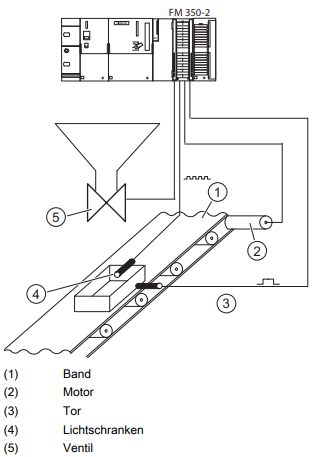
\includegraphics[width=0.8\textwidth]{Fotos/Beispiel_fm350-2.png}
    \caption{Beispiel für den Einsatz einer FM 350-2 in der S7-300 \cite{fm350_Handbuch}}
    \label{fig:fm350-2}
\end{figure}



%//////////////////////////////////////////////////////////////////////////////////////////////////////////////////////
%//////////////////////////////////////////////////////////////////////////////////////////////////////////////////////
\section{Vorteile und neue Möglichkeiten durch das TM FAST Modul} 

%//////////////////////////////////////////////////////////////////////////////////////////////////////////////////////
%//////////////////////////////////////////////////////////////////////////////////////////////////////////////////////
\section{Anforderungen an die Neuentwicklung} 


\begin{table}[h]
    \centering
    \renewcommand{\arraystretch}{1.3}
    \begin{tabularx}{\textwidth}{|X|X|X|}
        \hline
        \textbf{Kriterium} & \textbf{TM FAST} & \textbf{FM 350-2} \\
        \hline
        \multicolumn{3}{|c|}{\textbf{Unterschiede}} \\
        \hline
        Architektur & FPGA-basiert, flexible und programmierbare Hardwareplattform & Reines Zählermodul ohne FPGA-Technologie \\
        \hline
        Funktionalität & Kann komplexe Prozesssteuerungs- und Überwachungsaufgaben übernehmen & Spezialisiert auf Zählen, Frequenz- und Drehzahlmessung \\
        \hline
        Prozessintegration & Kann direkt in den Produktionsprozess eingreifen und Prozessalarme auslösen & Liefert Zähler- und Messwerte, die von der übergeordneten Steuerung weiterverarbeitet werden \\
        \hline
        Flexibilität & Hohe Flexibilität und Anpassungsfähigkeit durch FPGA-Architektur & Festgelegte Funktionalität, die nicht ohne Weiteres erweitert werden kann \\
        \hline
        \multicolumn{3}{|c|}{\textbf{Gemeinsamkeiten}} \\
        \hline
        Zählfunktionen & \multicolumn{2}{c|}{Beide Module bieten Zählfunktionen mit hoher Auflösung (z.B. 32-Bit Zähltiefe)} \\
        \hline
        Frequenz- und Drehzahlmessung & \multicolumn{2}{c|}{Beide Module unterstützen die Messung von Frequenzen und Drehzahlen} \\
        \hline
        Einbindung in Steuerungsarchitektur & \multicolumn{2}{c|}{Beide Module werden in die übergeordnete Steuerungsarchitektur integriert} \\
        \hline
        Industrielle Anwendungen & \multicolumn{2}{c|}{Beide Module finden Einsatz in ähnlichen Industriebereichen wie Verpackung, Sortierung, Dosierung etc.} \\
        \hline
    \end{tabularx}
    \caption{Vergleich zwischen TM FAST und FM 350-2}
    \label{tab:tm_fast_vs_fm350-2}
\end{table}

% \begin{table}[h]     funktioniert
%     \centering
%     \renewcommand{\arraystretch}{1.3} % Erhöht den Zeilenabstand leicht
%     \begin{tabularx}{\textwidth}{|X|X|X|}
%         \hline
%         \textbf{Kriterium} & \textbf{TM FAST} & \textbf{FM 350-2} \\\multicolumn{3}{|c|}{\textbf{Unterschiede}} \\
%         \hline
%         Architektur & FPGA-basiert, flexible und programmierbare Hardwareplattform & Reines Zählermodul ohne FPGA-Technologie \\
%         \hline
%         Funktionalität & Kann komplexe Prozesssteuerungs- und Überwachungsaufgaben übernehmen & Spezialisiert auf Zählen, Frequenz- und Drehzahlmessung \\
%         \hline
%         Prozessintegration & Kann direkt in den Produktionsprozess eingreifen und Prozessalarme auslösen & Liefert Zähler- und Messwerte, die von der übergeordneten Steuerung weiterverarbeitet werden \\
%         \hline
%         Flexibilität & Hohe Flexibilität und Anpassungsfähigkeit durch FPGA-Architektur & Festgelegte Funktionalität, die nicht ohne Weiteres erweitert werden kann \\
%         \hline
%     \end{tabularx}
%     \caption{Vergleich zwischen TM FAST und FM 350-2}
%     \label{tab:tm_fast_vs_fm350-2}
% \end{table}











\newif\ifdraft
%\drafttrue 
\draftfalse
\ifdraft

\chapter{Analyse der Ablösung des FM350-2 durch das TM FAST Modul}

\section{Funktionsweise und Limitierungen des FM350-2} 
\section{Vorteile und neue Möglichkeiten durch das TM FAST Modul} 
\section{Anforderungen an die Neuentwicklung} 



Unterschiede in der Aufgabe und Softwarearchetektur:

\begin{table}[h]
    \centering
    \renewcommand{\arraystretch}{1.3}
    \begin{tabularx}{\textwidth}{|X|X|X|}
        \hline
        \textbf{Kriterium} & \textbf{TM FAST} & \textbf{FM 350-2} \\
        \hline
        \multicolumn{3}{|c|}{\textbf{Unterschiede}} \\
        \hline
        Architektur & FPGA-basiert, flexible und programmierbare Hardwareplattform & Reines Zählermodul ohne FPGA-Technologie \\
        \hline
        Funktionalität & Kann komplexe Prozesssteuerungs- und Überwachungsaufgaben übernehmen & Spezialisiert auf Zählen, Frequenz- und Drehzahlmessung \\
        \hline
        Prozessintegration & Kann direkt in den Produktionsprozess eingreifen und Prozessalarme auslösen & Liefert Zähler- und Messwerte, die von der übergeordneten Steuerung weiterverarbeitet werden \\
        \hline
        Flexibilität & Hohe Flexibilität und Anpassungsfähigkeit durch FPGA-Architektur & Festgelegte Funktionalität, die nicht ohne Weiteres erweitert werden kann \\
        \hline
        \multicolumn{3}{|c|}{\textbf{Gemeinsamkeiten}} \\
        \hline
        Zählfunktionen & \multicolumn{2}{c|}{Beide Module bieten Zählfunktionen mit hoher Auflösung (z.B. 32-Bit Zähltiefe)} \\
        \hline
        Frequenz- und Drehzahlmessung & \multicolumn{2}{c|}{Beide Module unterstützen die Messung von Frequenzen und Drehzahlen} \\
        \hline
        Einbindung in Steuerungsarchitektur & \multicolumn{2}{c|}{Beide Module werden in die übergeordnete Steuerungsarchitektur integriert} \\
        \hline
        Industrielle Anwendungen & \multicolumn{2}{c|}{Beide Module finden Einsatz in ähnlichen Industriebereichen wie Verpackung, Sortierung, Dosierung etc.} \\
        \hline
    \end{tabularx}
    \caption{Vergleich zwischen TM FAST und FM 350-2}
    \label{tab:tm_fast_vs_fm350-2}
\end{table}

% \begin{table}[h]     funktioniert
%     \centering
%     \renewcommand{\arraystretch}{1.3} % Erhöht den Zeilenabstand leicht
%     \begin{tabularx}{\textwidth}{|X|X|X|}
%         \hline
%         \textbf{Kriterium} & \textbf{TM FAST} & \textbf{FM 350-2} \\\multicolumn{3}{|c|}{\textbf{Unterschiede}} \\
%         \hline
%         Architektur & FPGA-basiert, flexible und programmierbare Hardwareplattform & Reines Zählermodul ohne FPGA-Technologie \\
%         \hline
%         Funktionalität & Kann komplexe Prozesssteuerungs- und Überwachungsaufgaben übernehmen & Spezialisiert auf Zählen, Frequenz- und Drehzahlmessung \\
%         \hline
%         Prozessintegration & Kann direkt in den Produktionsprozess eingreifen und Prozessalarme auslösen & Liefert Zähler- und Messwerte, die von der übergeordneten Steuerung weiterverarbeitet werden \\
%         \hline
%         Flexibilität & Hohe Flexibilität und Anpassungsfähigkeit durch FPGA-Architektur & Festgelegte Funktionalität, die nicht ohne Weiteres erweitert werden kann \\
%         \hline
%     \end{tabularx}
%     \caption{Vergleich zwischen TM FAST und FM 350-2}
%     \label{tab:tm_fast_vs_fm350-2}
% \end{table}

\section{Funktionalität und Schnittstellen des FM350-2-Moduls}

\subsection{Funktionen}

\subsubsection{Die Funktion \texttt{FC CNT2\_CTR} (FC2), Baugruppe steuern}

\begin{itemize}
    \item \textbf{Aufgabe: } Mit der \texttt{FC CNT2\_CTR} steuern Sie die Digitalausgänge (Freigabe und Sperrung) sowie die Software-Tore der FM 350-2. Außerdem erhalten Sie Rückmeldungen von der FM 350-2.
    \item \textbf{Aktion: } Die \texttt{FC CNT2\_CTR} führt folgende Aktionen durch: 
                            \subitem 1. Zähler-DB initialisieren 
                            \subitem 2. Lesen der Rückmeldesignale. Die gelesenen Werte werden vom FC im Zähler-DB in der 
                            Struktur CHECKBACK\_SIGNALS abgelegt. 
                            \subitem 3. Übertragen der Steuersignale aus dem Zähler-DB (Struktur CONTROL\_SIGNALS) zur 
                            FM 350-2.
    \item \textbf{Aufruf: } Sie müssen die \texttt{FC CNT2\_CTR} zyklisch (im OB1 oder in den Weckalarmen - nur OB35 in 
    S7-300) für jede Baugruppe aufrufen. Der Aufruf in einem Alarmprogramm ist nicht zulässig. 
    Vor dem Aufruf der \texttt{FC CNT2\_CTR} tragen Sie die aktuellen Steuersignale in der Struktur 
    CONTROL\_SIGNALS im Zähler-DB ein. Nach dem Aufruf der \texttt{FC CNT2\_CTR} sind die 
    Rückmeldesignale in der Struktur CHECKBACK\_SIGNALS im Zähler-DB aktualisiert und Sie 
    können diese von dort weiterverarbeiten. 
    Die Nummer des Zähler-DBs wird beim Aufruf des FC an dem Parameter DB\_NO 
    angegeben.
\end{itemize}

\subsubsection{Zählerstände, Grenzwerte und Vergleichswerte laden (\texttt{FC3} / \texttt{FB3})}

Mit der \texttt{FC CNT2\_WR} / \texttt{FB CNT2WRPN} laden Sie die Zähler und Vergleicher der FM 350-2 
mittels Schreibaufträgen. Dazu müssen Sie die \texttt{FC CNT2\_WR} / \texttt{FB CNT2WRPN} bei Bedarf 
pro Baugruppe aufrufen.  
Sie binden die Funktion \texttt{FC CNT2\_WR} / \texttt{FB CNT2WRPN} nur in Ihr Programm ein, wenn Sie 
die Zähler und Vergleicher der FM 350-2 im Betrieb neu laden müssen.
 
\subsection{Zähl- und Messwerte auslesen (\texttt{FC4} / \texttt{FB4})}

Mit der \texttt{FC CNT2\_RD} / \texttt{FB CNT2RDPN} lesen Sie Zähl- und Messwerte von der FM 350-2 
mit Leseaufträgen. Dazu rufen Sie die \texttt{FC CNT2\_RD} / \texttt{FB CNT2RDPN} zyklisch einmal pro 
Baugruppe auf.  
Sie binden die \texttt{FC CNT2\_RD} / \texttt{FB CNT2RDPN} nicht in Ihr Anwenderprogramm ein, wenn 
Sie keine Leseaufträge bearbeiten.

\subsection{Die Funktion \texttt{FC DIAG\_RD} (FC5), Diagnosedaten lesen}

Mit der \texttt{FC DIAG\_RD} können Sie im Falle eines Diagnosealarms die Diagnosealarmdaten in 
den Zähler-DB laden.


\section{Einsatzgebiete der FM 350-2 / evtl nicht nötig}

\subsection{Haupteinsatzgebiet} Das Haupteinsatzgebiet der FM 350-2 liegt dort, wo Signale gezählt und schnelle Reaktionen auf einen vorgegebenen Zählerstand ausgelöst werden müssen sowie Frequenzen oder Drehzahlen gemessen werden sollen.

\subsection{Beispiele für den Einsatz} Beispiele hierfür sind: \begin{itemize} \item Verpackungsanlagen \item Sortieranlagen \item Dosieranlagen \item Drehzahlregelungen und Überwachung von Gasturbinen \end{itemize}

\subsection{Beispiel für den Einsatz einer FM 350-2} Aus einem Sammelbehälter soll eine bestimmte Anzahl Teile in einen Karton abgefüllt werden. Der Zählkanal 0 zählt die Teile und steuert das Ventil zur Abfüllung. Mit dem Zählkanal 1 wird der Motor zum Transport der Kartons gesteuert und die Anzahl der Kartons gezählt.

Befindet sich der Karton in der richtigen Position wird das Ventil geöffnet und die Teile werden abgefüllt. Ist die vorgegebene Anzahl erreicht, wird das Ventil geschlossen und der Transport des Kartons angestoßen. Nachfallende Teile werden mitgezählt bis ein neuer Karton eintrifft.
Während des Transports der Kartons ist eine neue Anzahl Teile vorgebbar. Die abgefüllten Teile sowie die Anzahl der Kartons ist beobachtbar. 
\fi